\documentclass{beamer}
\usepackage{tfrupee} 
\usepackage[utf8]{inputenc}
\usepackage{lmodern} 
\usepackage[utf8]{inputenc}
\usepackage{lmodern} 
\usepackage{listings}
\usepackage{xcolor} 
\usepackage{graphicx}
\definecolor{myblue}{RGB}{48, 63, 159}
\setbeamercolor{palette primary}{bg=myblue, fg=white}
\setbeamercolor{structure}{fg=myblue}
\setbeamercolor{frametitle}{bg=myblue, fg=white}
\setbeamercolor{title}{bg=myblue, fg=white}
\setbeamercolor{footlinecolor}{bg=myblue, fg=white}


\defbeamertemplate*{title page}{mytemplate}{
	\vfill
	\begin{center}
		
		\begin{beamercolorbox}[wd=0.8\paperwidth, center, rounded=true, shadow=true]{title}
			\usebeamerfont{title}\inserttitle\par
		\end{beamercolorbox}
		\vspace{2cm} 
		
		\usebeamerfont{author}\insertauthor
		\vspace{1cm} 
		\usebeamerfont{date}\insertdate
	\end{center}
	\vfill
}


\defbeamertemplate*{frametitle}{mytemplate}{
	\begin{beamercolorbox}[wd=\paperwidth, ht=2.5ex, dp=1.5ex, left]{frametitle}
		\hspace{1em}\usebeamerfont{frametitle}\insertframetitle
	\end{beamercolorbox}
}


\setbeamertemplate{footline}{
	\begin{beamercolorbox}[wd=\paperwidth, ht=2.25ex, dp=1ex]{footlinecolor}
		\hspace{1em}\usebeamerfont{author in footline}\insertshortauthor
		\hfill
		\usebeamerfont{title in footline}\insertshorttitle
		\hfill
		\usebeamerfont{date in footline}\insertdate \hspace{1em} \insertframenumber/\inserttotalframenumber \hspace{0.5em}
	\end{beamercolorbox}
}


\setbeamerfont{author in footline}{size=\tiny}
\setbeamerfont{title in footline}{size=\tiny}
\setbeamerfont{date in footline}{size=\tiny}

\newcommand{\myvec}[1]{\ensuremath{\begin{pmatrix}#1\end{pmatrix}}}
\providecommand{\brak}[1]{\ensuremath{\left(#1\right)}}


\title{9.2.15}
\author{Shriyansh Chawda-EE25BTECH11052}




\begin{document}
	

		\setbeamertemplate{footline}{} 
		\frame{\titlepage}
	
	
\begin{frame}{Question} 
Determine the area under the curve $y = \sqrt{a^2 - x^2}$ included above the  x axis.\\
\end{frame}
	
\begin{frame}{Solution}
General Equation of Conic in Matrix form is given by :
\begin{equation}
	\mathbf{x}^\top\mathbf{V}\mathbf{x} + 2\mathbf{u}^\top\mathbf{x} + f = 0
	\label{eq:matrix_conic}
\end{equation}
First,The  curve $y = \sqrt{a^2 - x^2}$ can be Rearranged as : 
\begin{align}
	y^2 = a^2 - x^2 \implies x^2 + y^2 - a^2 = 0
\end{align}
Using this, The specific conic parameters for this curve:
\begin{equation}
	\mathbf{V} = \myvec{1 & 0 \\ 0 & 1}, \quad \mathbf{u} = \myvec{0 \\ 0}, \quad f = -a^2
\end{equation}
Next, the area is bounded below by the x-axis (the line $y=0$). The parameters for this line are:
\begin{equation}
	\mathbf{h} = \myvec{0 \\ 0}, \quad \mathbf{m} = \myvec{1 \\ 0}
\end{equation}
\end{frame}



\begin{frame}{Solution}
Using the formula given in the  book to solve point of intersection of line with a given curve:

\[
\kappa = \frac{1}{\mathbf{m}^\top\mathbf{V}\mathbf{m}} \left( -\mathbf{m}^\top(\mathbf{V}\mathbf{h} + \mathbf{u}) \pm \sqrt{ (\mathbf{m}^\top(\mathbf{V}\mathbf{h} + \mathbf{u}))^2 - g(\mathbf{h})(\mathbf{m}^\top\mathbf{V}\mathbf{m}) } \right)
\]
where $g(\mathbf{h}) = \mathbf{h}^\top\mathbf{V}\mathbf{h} + 2\mathbf{u}^\top\mathbf{h} + f$. We calculate each component:
\begin{align}
	&\mathbf{m}^\top\mathbf{V}\mathbf{m} = \myvec{1 & 0} \myvec{1 & 0 \\ 0 & 1} \myvec{1 \\ 0} = \myvec{1 & 0} \myvec{1 \\ 0} = 1\\
	&\mathbf{m}^\top(\mathbf{V}\mathbf{h} + \mathbf{u}) = \myvec{1 & 0} \left( \myvec{1 & 0 \\ 0 & 1} \myvec{0 \\ 0} + \myvec{0 \\ 0} \right) = \myvec{1 & 0} \myvec{0 \\ 0} = 0\\
	&g(\mathbf{h}) = \myvec{0 & 0}\myvec{1 & 0 \\ 0 & 1}\myvec{0 \\ 0} + 2\myvec{0 & 0}\myvec{0 \\ 0} - a^2 = 0 + 0 - a^2 = -a^2
\end{align}
\end{frame}

\begin{frame}{Solution}
Substituting these results back into the formula for $\kappa$:
\[
\kappa = \frac{1}{1} \left( -0 \pm \sqrt{ (0)^2 - (-a^2)(1) } \right) = \pm \sqrt{a^2} = \pm a
\]
The solutions are $\kappa_1 = a$ and $\kappa_2 = -a$, confirming the intersections at $x=\pm a$.

Hence,The area can be given by :
\begin{align}
	A = \int_{-a}^{a} \sqrt{a^2 - x^2} dx
\end{align}


This integral is solved using trigonometric substitution. Let $x = a \sin\theta$, so $dx = a \cos\theta \,d\theta$. The limits become $-\frac{\pi}{2}$ to $\frac{\pi}{2}$.
\end{frame}
\begin{frame}{Solution}
\begin{align}
	A &= \int_{-\frac{\pi}{2}}^{\frac{\pi}{2}} \sqrt{a^2 - a^2\sin^2\theta} \cdot (a \cos\theta \,d\theta) \\
	&= \int_{-\frac{\pi}{2}}^{\frac{\pi}{2}} \sqrt{a^2\cos^2\theta} \cdot (a \cos\theta \,d\theta) \\
	&= \int_{-\frac{\pi}{2}}^{\frac{\pi}{2}} (a \cos\theta) (a \cos\theta \,d\theta) \\
	&= a^2 \int_{-\frac{\pi}{2}}^{\frac{\pi}{2}} \cos^2\theta \,d\theta \\
	&= a^2 \int_{-\frac{\pi}{2}}^{\frac{\pi}{2}} \frac{1 + \cos(2\theta)}{2} \,d\theta \\
	&= \frac{a^2}{2} \left[ \theta + \frac{1}{2}\sin(2\theta) \right]_{-\frac{\pi}{2}}^{\frac{\pi}{2}} 
\end{align}
\end{frame}

\begin{frame}{Solution}
\begin{align}
	&= \frac{a^2}{2} \left( \left[ \frac{\pi}{2} + \frac{1}{2}\sin(\pi) \right] - \left[ 0 + \frac{1}{2}\sin(-\frac{\pi}{2}) \right] \right) \\
&= \frac{a^2}{2} \left( \frac{\pi}{2} \right) = \frac{\pi a^2}{2}
\end{align}
\end{frame}

\begin{frame}{Plot}
\begin{figure}[H]
	\centering
	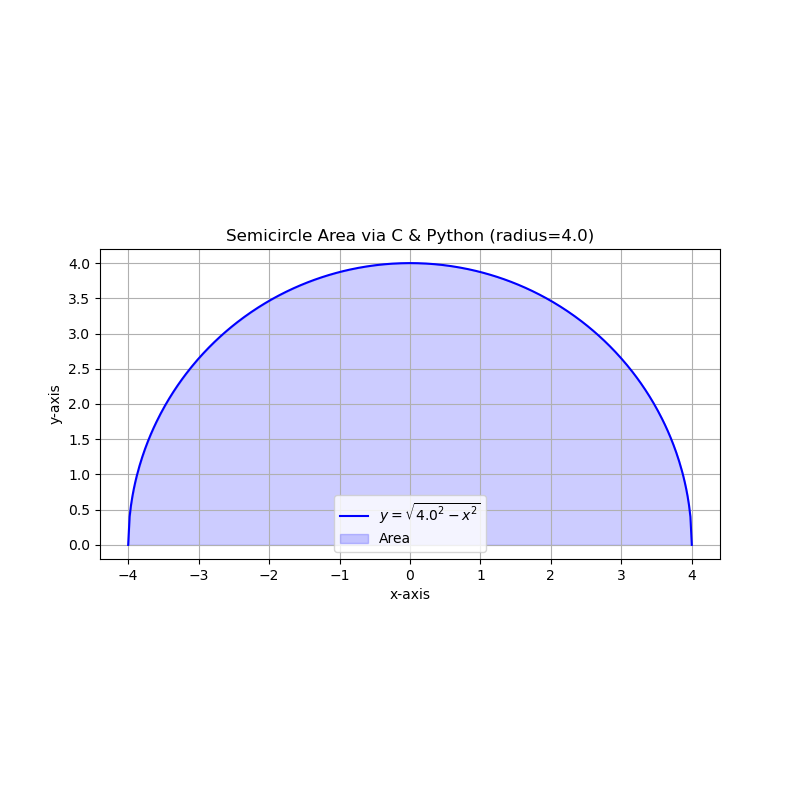
\includegraphics[width=1\linewidth]{../figs/semicircle_plot_from_c}
\end{figure}

\end{frame}


\end{document}